\section{Aufgabe 2: Neuronale Netze}
\subsection{Neuronale Netze mit Numpy}
\subsubsection{Implementierung Backprop mit einem Hidden Layer}
Die Herleitung der Backpropagation basiert auf der Kostenfunktion, die den Fehler der Output Schicht beschreibt, sowie den Definitionen der einzelnen Gradienten. Die Definition der Fehlerfunktion, sowie die Variablennamen und Indizes wurden aus der Aufgabenstellung übernommen. Es wird mit den Gewichten zwischen dem Hidden und dem Output Layer gestartet (d$W_{2}$), da nur für die Output Schicht ein messbarer Fehler vorliegt. Im ersten Schritt wird die Kostenfunktion in die  Definition d$W_{2}$ eingesetzt und anschließend die partielle Ableitung gebildet.
\begin{align*}
dW_{2} &= \frac{\partial E}{\partial W_{2}}
= \frac{\partial E}{\partial z_{2}}\cdot \frac{\partial z_{2}}{\partial W_{2}}
\end{align*}
Diese teilt sich auf in ein $\delta_{2}$, welches den Fehler und die abgeleitete Aktivierungsfunktion enthält, und den Outputs der Hidden Schicht ($a_{1}$).
\begin{align*}
\frac{\partial E}{\partial z_{2}}\cdot \frac{\partial z_{2}}{\partial W_{2}} = \delta_{2} \cdot a_{1}= -(y-\hat{\pi}) \cdot \sigma(a_{1}W_{2}+b_{2})(1-\sigma(a_{1}W_{2}+b_{2}))\cdot a_{1}
\end{align*}
Für die Gewichte des Bias der Hidden Schicht (d$b_{2}$) wird der Output-Term durch 1 ersetzt, da dieser für den Bias immer konstant 1 beträgt.
\begin{align*}
db_{2} &= \frac{\partial E}{\partial b_{2}}
= \delta_{2} \cdot 1 = -(y-\hat{\pi}) \cdot \sigma(a_{1}W_{2}+b_{2})(1-\sigma(a_{1}W_{2}+b_{2})) \cdot 1
\end{align*}
Für die Gradienten zwischen der Input Schicht und der Hidden Schicht wir das gleiche Vorgehen genutzt. Da kein direkter Fehler gemessen werden kann, wird der Fehler-Term durch den backpropagierten gewichteten Fehler der Output Schicht ersetzt.
\begin{align*}
dW_{1} &= \frac{\partial E}{\partial W_{1}}
= \frac{\partial E}{\partial z_{2}}\cdot \frac{\partial z_{2}}{\partial z_{1}} \cdot X = \delta_{2} \cdot \frac{\partial z_{2}}{\partial z_{1}} \cdot X
\end{align*}
Dieser gewichtete Fehler ergibt sich aus dem $\delta$ der jeweils nachfolgenden Schicht (hier $\delta_{2}$). Der Output-Term der vorherigen Schicht entspricht hier den Inputs ($X$), die durch die Stichprobendaten gegeben sind, sodass gilt:
\begin{align*}
dW_{1} &= \delta_{2}\cdot W_{2} \cdot \sigma(X\cdot W_{1}+b_{1})(1- \sigma(X\cdot W_{1}+b_{1})) \cdot X
\end{align*}
\noindent
Wobei für $db_{1}$ statt $X$ wieder 1 eingesetzt wird. In Anhang \ref{app:ergaenzung_booklet_2} ist die ausführliche mathematische Ausarbeitung des beschriebenen Vorgehens zu finden. Zusätzlich findet sich in Anhang \ref{app:quellcode_booklet_2} die dazugehörige Python-Implementierung.
\subsubsection{Hyperparameter}
Im Folgenden werden Hyperparameter beschrieben, sowie ihre Auswirkungen auf das neuronale Netzwerk diskutiert.
\begin{description}
	\item[Anzahl der Neuronen im Hidden Layer]\hfill \\
	%TODO: Eigentlcih sollte der Fehler auf die Trainingsdaten bei vielen Neuronen minimal sein. Irgendwie overfittet das Modell nicht klassisch.
	Wenn keine $l_1$ oder $l_2$ Regularisierung, Dropout \cite{dropout} oder andere Regularisierungstechniken eingesetzt werden, steigt die Gefahr einer Überanpassung mit steigender Anzahl an Neuronen im Netzwerk. Werden zu wenige Neuronen im Hidden Layer eingesetzt, steigt hingegen die Gefahr einer Unteranpassung. In der Praxis wählt man eher ein Netzwerk mit zu vielen Neuronen in den Hidden Layern und wirkt Overfitting mit Hilfe von Regularisierungstechniken entgegen \cite{geron2017hands-on}. Tabelle \ref{table:overfitting} zeigt den Netzwerkfehler abhängig von der Anzahl an Neuronen im Hidden Layer. Anhand der beobachteten Werte aus der Tabelle kann man jedoch nicht auf ein Overfitting bei steigender Neuronen-Anzahl schließen. Denn ab einer Neuronen-Anzahl von 100 steigt der Fehler auf die Trainingsdaten ebenso, wie der Fehler auf die Testdaten. Es ist eher zu beobachten, dass das Netzwerk mit steigender Neuronen Anzahl generell Schwierigkeiten hat, den Fehler zu minimieren.
	\begin{table}[ht]
		\centering
		\begin{tabular}{l|llllll}
			& 10000 & 1000 & 100  & 10   & 5    & 2    \\ \hline
			Test Fehler      & 62    & 19,9 & 14,9 & 14.9 & 14.9 & 15   \\
			Trainings Fehler & 188   & 43,5 & 35,1 & 35,0 & 35,0 & 35,1
		\end{tabular}
		\caption{\label{table:overfitting}Netzwerkfehler abhängig von der Anzahl an Neuronen im Hidden Layer.}
	\end{table}
	
	\item[Anzahl an Iterationen]\hfill \\
	Die Anzahl der Iterationen, die benötigt werden, bis der Trainingsfehler nicht mehr sinkt, hängt stark von der gewählten Lernrate ab. Im weiteren Verlauf wird das einmalige Iterieren durch den gesamten Trainingsdatensatz als Epoche bezeichnet. In Abbildung \ref*{fig:learning_rates} ist der Trainingsverlauf während mehrerer Epochen für verschiedene Lernraten abgebildet. Bei einer Lernrate von 0.1 sinkt der Trainingsfehler nach 100 Epochen nicht mehr. Sobald der Trainingsfehler während mehrerer aufeinanderfolgenden Epochen nicht weiter sinkt, sollte das Training beendet werden, da sonst die Gefahr von Overfitting steigt.
	
	\item[Lernrate]\hfill \\
	Die Lernrate $\eta$ reguliert die Auswirkung eines einzelnen Schrittes im Gradientenabstiegsverfahrens. Eine hohes $\eta$ führt zwar zu einer schnellen Minimierung des Trainingsfehlers, jedoch steig die Gefahr, dass das Verfahren gute Minima überspringt oder auch um ein gutes Minima pendelt. Ein kleineres $\eta$ findet mit einer hohen Wahrscheinlichkeit ein besseres Minima, jedoch werden dafür mehr Iterationen und damit auch mehr Rechenleistung benötigt \cite{neuronalenetze}.\\
	\noindent \hspace*{7mm}
	In Abbildung \ref*{fig:learning_rates} ist der Trainingsfehler während des Trainingsverlauf bei verschiedenen Lernraten dargestellt. Der Abbildung kann entnommen werden, dass für $\eta=0.01$ das Training nach 300 Epochen immer noch nicht konvergiert ist. Für $\eta=0.2$ ist zu sehen, dass das Verfahren sehr früh konvergiert und daher das Risiko besteht, dass wie oben beschrieben gute Minima übersprungen wurden. Für komplexere Eingabedaten und Netzwerkarchitekturen würde dies ein reales Problem darstellen. In diesem einfachen Netzwerk und den einfachen Eingabedaten aus der Aufgabenstellung, kann auch mit $\eta=0.2$ ein gutes Ergebnis erreicht werden. Der Mittelweg beider Extreme bildet $\eta=0.1$ und wird als Einstellung vorgenommen.
	
	\begin{figure}[ht]
		\centering
		\vspace*{-0.9 cm}
		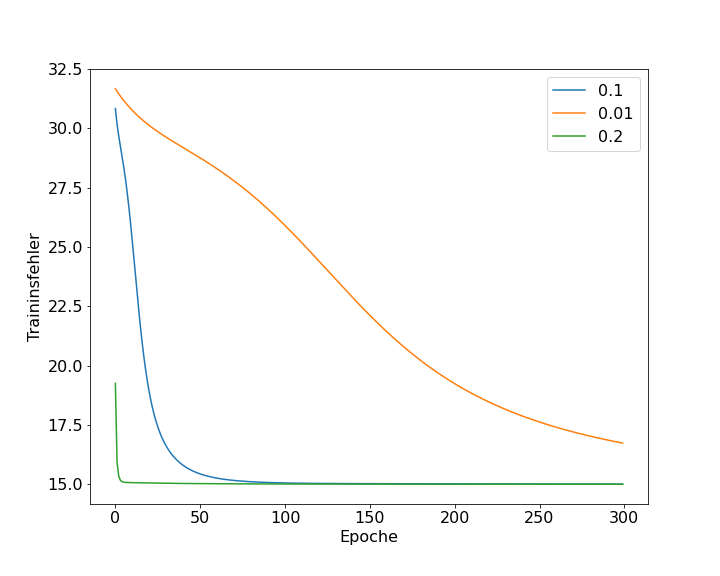
\includegraphics[width = 0.45\textwidth]{Bilder/learning_rates.png}
		\caption{Trainingsfehler während der Trainingsepochen bei verschiedenen Lernraten}
		\label{fig:learning_rates}
	\end{figure}
	
	\item[Initialisierung der Gewichte]\hfill \\
	Vor Allem beim Trainieren von tiefen neuronalen Netzen spielt die Initialisierung der Gewichte eine entscheidende Rolle, um das Auftreten des Problems der explodierenden beziehungsweise verschwindenden Gradienten entgegen zu wirken \cite{geron2017hands-on}. In \cite{Glorot10understandingthe} wird die Glorot-Initialisierung, ein Verfahren zur Initialisierung der Gewichte bei Verwendung der Sigmoid Aktivierungsfunktion, beschrieben. Hierbei werden die Werte der initialen Gewichte aus einer Normalverteilung $\mathcal{N}(\mu,\,\sigma^{2})\,$ mit $\mu = 0$ und $\sigma^{2}=\frac{1}{fan_{avg}}$ entnommen. Hierbei gilt: 
	\[
	fan_{avg}=\frac{(fan_{in}+fan_{out})}{2}
	\]
	Wobei $fan_{in}$ der Anzahl an eingehenden Gewichte in einer Schicht entspricht und  $fan_{out}$ der Anzahl an Neuronen in der Schicht. Die Initialisierung der Gewichte in der vorliegenden Arbeit wurde  nach Glorot implementiert. Die Gewichte der Biase wurden mit 0 initialisiert.\\
	\noindent \hspace*{7mm}
	Würden die Gewichte mit Null initialisiert werden, würde der Gradient für alle Schichten, bis auf die Ausgabeschicht, Null sein. Ein Lernen würde daher nur sehr begrenzt stattfinden. Der Gradient für die Aktualisierung der Gewichte zwischen versteckter Schicht und Ausgabeschicht würde für alle partiellen Ableitungen gleich sein. Auch eine Initialisierung mit einer anderen Konstanten würde dazu führen, dass alle Gewichte in einer Schicht gleich aktualisiert werden würden. Sie könnten dann auch einfach durch ein einzelnes Neuron mit einer einzigen Verbindung ersetzt werden.\\
	\noindent\hspace*{7mm}
	Mithilfe der Verwendung eines \emph{Seeds} wird sicher gestellt, dass die zufällige Initialisierung der Gewichte bei jedem Durchlauf mit den gleichen Parametern die gleichen zufälligen Werte liefert. Das Netzwerk liefert also mit jedem Durchlauf bei gleichen Daten und Parametern die gleichen Ergebnisse. Somit wird die Reproduzierbarkeit im Netzwerk gefördert, was bei einer Fehlersuche und der Hyperparameter Optimierung hilfreich sein kann.
	
\end{description}
\subsection{Neuronale Netze mit TensorFlow}
%TODO: Beschreiben, welche Daten zum Trainieren genommen wurden
Im Folgenden wird die Implementierung eines voll vernetzen neuronalen Netzwerks mit Hilfe der \emph{TensorFlow} Bibliothek beschrieben \cite{tensorflow2015-whitepaper}. Unterstützend wurde für den Aufbau des neuronalen Netzes die \emph{Keras}-API verwendet, die seit \emph{TensorFlow} Version 2 standardmäßig integriert ist. \\
\noindent \hspace*{7mm}
Um die Daten für das Training des neuronalen Netzes effizient vorzubereiten, wurde die \emph{Dataset}-API verwendet. Mit Hilfe der \emph{Dataset}-API wurde das zufällige Mischen der Trainingsdaten, sowie die Bereitstellung in Form von \emph{Mini-Batches} implementiert. Die Verwendung der \emph{Dataset}-API hat noch zusätzlich den Vorteil, dass die Ausführung von Vorbereitungsschritten der Daten perfekt mit dem Training des neuronalen Netzes koordiniert und parallelisiert werden können.

\subsubsection{Hyperparameter Suche}
\label{nn_hyperparams}
Um ein optimales Modell für die vorliegenden Daten zu finden, wurde eine automatisierte Suche nach den besten Hyperparameter-Kombination implementiert. Die zur Auswahl stehenden Hyperparameter mit ihren möglichen Ausprägungen sind in Tabelle \ref{table:hyper} aufgeführt.

\begin{table}[ht]
	\centering
	\begin{tabular}{ll}
		\textbf{Hyperparameter}     & \textbf{Ausprägungen} \\ \hline
		Anzahl Hidden Layer         & 0,1,2,3,4             \\
		Anzahl Neuronen pro Schicht & 1,3,5,10,20,50,100    \\
		Lernrate                    & 0,1;  0,05;  0.01     \\
		Aktivierungsfunktion        & ReLU, Sigmoid, ELU \\
		Dropout Wahrscheinlichkeit  & 0;  0.25;  0.5       
	\end{tabular}
	\caption{\label{table:hyper} Parameterraum der Hyperparameter Suche}
\end{table}

Durch begrenzte Ressourcen wäre eine Evaluierung aller möglichen Hyperparameter-Kombinationen mittels einer \emph{Grid Search} nicht möglich. In der vorliegenden Arbeit wurde deshalb eine zufällige Suche nach \cite{randomSearch} implementiert. Das Sieger-Modell aus 10 zufälligen Hyperparameter-Kombinationen besteht aus 4 Hidden Layern mit jeweils 3 Neuronen. Die Lernrate wurde auf 0.1 festgelegt und das Netzwerk wurde ohne die Verwendung von Dropout trainiert. Als effektivste Aktivierungsfunktion hat sich die ELU-Funktion herausgestellt \cite{elu}. Das Sieger-Modell konnte eine Klassifizierungsgenauikgkeit von 85,11\% auf die Testdaten erreichen. Die Daten zum Trainieren und Testen des neuronalen Netzwerks wurden analog zu Aufgabenstellung \ref{section:Entscheidungsbäume} verwendet. Im Vergleich zu der Klassifizierungsgenauigkeit des Entscheidungsbaums aus \ref{variation_tree} schneidet das entworfene neuronale Netzwerk um 0,61 Prozentpunkte besser ab. Der Nachteil des neuronalen Netzwerks ist jedoch, dass die Entscheidungskriterien im Vergleich zum Entscheidungsbaum nur sehr schwer interpretierbar sind.
